The final array contains the numerical value of the electric potential at each point in the grid as a number of type \lstinline|double|. The program outputs the value of each point along the $y$-direction corresponding to an $x$ value, then moves on to the next $x$ value and repeats the process. The program writes the value of the potential at each point to a file in the format shown in table \ref{tab:potential_data}.

An output file is also produced to allow the plotting of the electric field. The file contains the $x$ and $y$ coordinates as well as the $d{\phi}/dx$ and $d{\phi}/dy$ values, which are approximated using central differencing. The values are then written to a file in the format shown in table \ref{tab:field_data}.
\begin{table}
\parbox{0.47\linewidth}{
\centering
\begin{tabularx}{0.44\textwidth}{ |XXX| }
\hline
$x_1$ & $y_1$ & $\phi_{1,1}$ \\
$x_1$ & $y_2$ & $\phi_{1,2}$ \\
$x_1$ & $y_3$ & $\phi_{1,3}$ \\
& & \\
$x_2$ & $y_1$ & $\phi_{2,1}$ \\
$x_2$ & $y_2$ & $\phi_{2,2}$ \\
$x_2$ & $y_3$ & $\phi_{2,3}$ \\
& & \\
$x_3$ & $y_1$ & $\phi_{3,1}$ \\
$x_3$ & $y_2$ & $\phi_{3,2}$ \\
$x_3$ & $y_3$ & $\phi_{3,3}$ \\
\hline
\end{tabularx}
\caption{Structure of a file containing information about the potential across the grid. This example is for a 3x3 grid.}
\label{tab:potential_data}
}
\hfill
\parbox{0.47\linewidth}{
\centering
\begin{tabularx}{0.44\textwidth}{ |XXXX| }
\hline
$x_1$ & $y_1$ & $d{\phi}/dx_{1,1}$ & $d{\phi}/dy_{1,1}$ \\
$x_1$ & $y_2$ & $d{\phi}/dx_{1,2}$ & $d{\phi}/dy_{1,2}$ \\
$x_1$ & $y_3$ & $d{\phi}/dx_{1,3}$ & $d{\phi}/dy_{1,3}$ \\
& & & \\
$x_2$ & $y_1$ & $d{\phi}/dx_{2,1}$ & $d{\phi}/dy_{2,1}$ \\
$x_2$ & $y_2$ & $d{\phi}/dx_{2,2}$ & $d{\phi}/dy_{2,2}$ \\
$x_2$ & $y_3$ & $d{\phi}/dx_{2,3}$ & $d{\phi}/dy_{2,3}$ \\
& & & \\
$x_3$ & $y_1$ & $d{\phi}/dx_{3,1}$ & $d{\phi}/dy_{3,1}$ \\
$x_3$ & $y_2$ & $d{\phi}/dx_{3,2}$ & $d{\phi}/dy_{3,2}$ \\
$x_3$ & $y_3$ & $d{\phi}/dx_{3,3}$ & $d{\phi}/dy_{3,3}$ \\
\hline
\end{tabularx}
\caption{Structure of a file containing information about the electric field across the grid. This example is for a 3x3 grid.}
\label{tab:field_data}
}
\end{table}
The data can then be plotted as a vector field in gnuplot using ``plot \ldots with vectors". By setting some functions in gnuplot, the vectors in the field can be made of uniform size and coloured to indicate the magnitude of the vector. Equipotential lines can be overlaid on the plot. The equipotential lines are drawn by the contour function in gnuplot. An example of an equipotential line plot overlaid on a vector field can be seen in Figure
\ref{fig:vectors_and_contours}.
\begin{figure}[h!]
\centering
\setlength\fboxsep{0pt}
\setlength\fboxrule{0.5pt}
\fbox{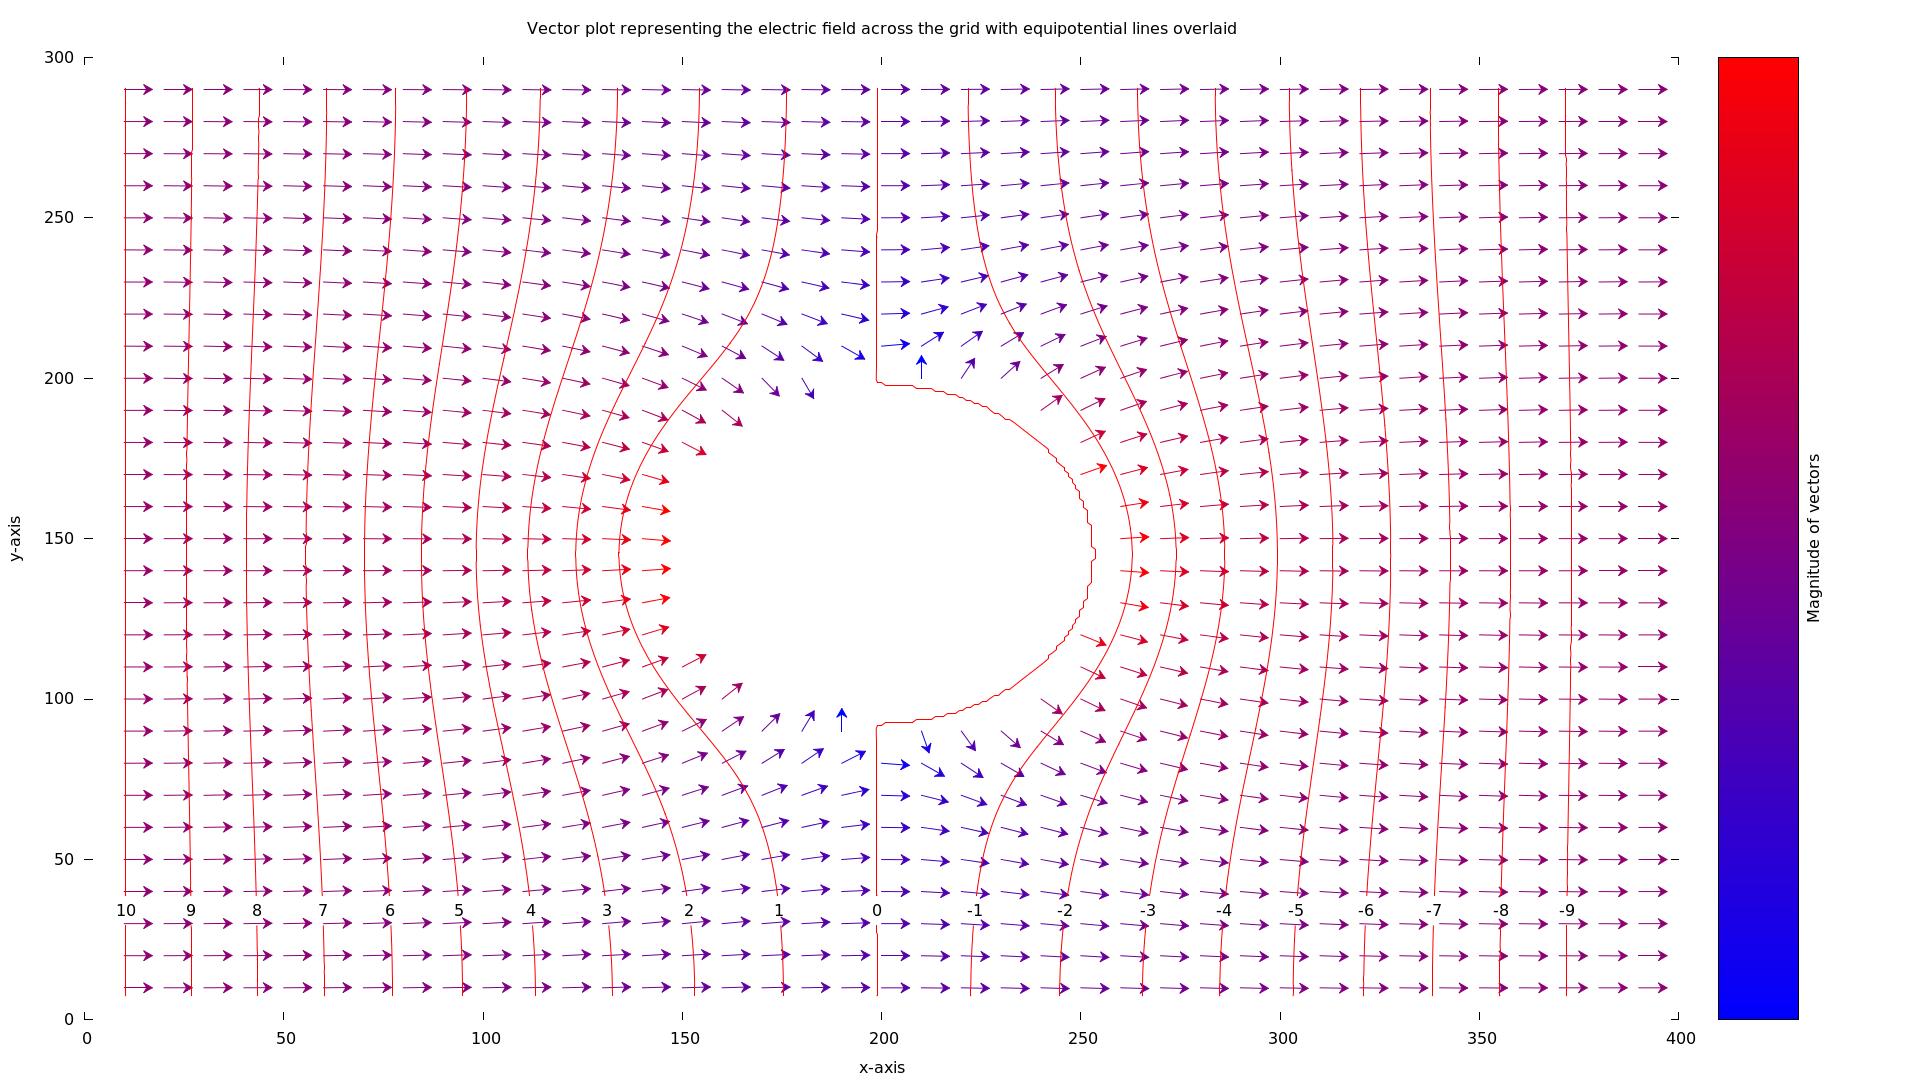
\includegraphics[width=0.95\textwidth, trim = 0mm 0mm 0mm 0mm, clip]{example_vectors_and_contours.png}} % trim options: left bottom right top, change to appropriate values if some other image is used and it has too much whitespace around it.
\caption{A plot displaying the electric field represented as vectors with equipotential lines overlaid on top of them.}
\label{fig:vectors_and_contours}
\end{figure}
All of the plotting in the program is done internally via C++ functions which call gnuplot to be run.
